\documentclass[sigconf]{acmart}

% \usepackage{booktabs} % For formal tables

% \makeatletter
% \def\@ACM@printacmref\false
% \makeatother

\settopmatter{printacmref=false} % アブストラクトの下のRef情報を表示しあい

\usepackage{graphicx}
\usepackage{here} % [H]とするとその場所に配置されるらしい

% Copyright
%\setcopyright{none}
%\setcopyright{acmcopyright}
%\setcopyright{acmlicensed}
\setcopyright{rightsretained}
%\setcopyright{usgov}
%\setcopyright{usgovmixed}
%\setcopyright{cagov}
%\setcopyright{cagovmixed}


% % DOI
% \acmDOI{10.475/123_4}
% 
% % ISBN
% \acmISBN{123-4567-24-567/08/06}
% 
% Conference
\acmConference[AVI2018]{International Conference on Advanced Visual Interfaces}{May 2018}
              {Resort Riva del Sole, Castiglione della Pescaia, Grosseto (Italy)}
\acmYear{2018}
\copyrightyear{2018}
\acmISBN{}
\acmDOI{}
% 
% 
% \acmArticle{4}
% \acmPrice{15.00}

% These commands are optional
%\acmBooktitle{Transactions of the ACM Woodstock conference}
% \editor{Jennifer B. Sartor}
% \editor{Theo D'Hondt}
% \editor{Wolfgang De Meuter}

\begin{document}
\title{EpisoDAS - DAS-based Password Generation \\
using Episodic Memories}
% \titlenote{Produces the permission block, and copyright information}

\author{xxxxxx xxxx}
% \authornote{Is this necessary?.}
% \orcid{1234-5678-9012}
\affiliation{%
  % \institution{Keio University}
  % \streetaddress{5322 Endo}
  % \city{Fujisawa}
  % \state{Kanagawa}
  % \postcode{252-8520}
  \institution{xxxxxx xxxxxx}
  \streetaddress{xxxx xxxx}
  \city{xxxxxxx}
  \state{xxxxxxx}
  \postcode{00000000}
}
% \email{masui@masui.org}
\email{xxxx@xxxxx.xxxx}

% \renewcommand{\shortauthors}{T. Masui}

\begin{CCSXML}
  <ccs2012>
  <concept>
  <concept_id>10002978.10002991.10002992.10011618</concept_id>
  <concept_desc>Security and privacy~Graphical / visual passwords</concept_desc>
  <concept_significance>500</concept_significance>
  </concept>
  </ccs2012>
\end{CCSXML}
\ccsdesc[500]{Security and privacy~Graphical / visual passwords}

\keywords{Passwords; visual passwords; user authentication;
  episodic memories; draw-a-secret.}

\begin{abstract}

We introduce a simple and powerful visual interaction technique for
managing strong passwords.
%
Passwords have been used for authentication for decades, but
appropriate handling of passwords is difficult because people can
easily forget passwords and they can be easily attacked.
%
To make the authentication process easier, various visual interaction
methods have been proposed, including the DAS (draw-a-secret)
method. Using DAS, users can log into various services just by drawing
a secret pattern on the screen.
%
Using a DAS-based authentication method, users can quickly log into a
service without typing a password, but remembering complex secret
patterns is as difficult as remembering passwords.
%
We developed \textit{EpisoDAS}, with which users can generate strong passwords
based on their secret episodic memories with a simple DAS interface.
%
users can use secret patterns for authentication, based on their
secret episodic memories that they cannot easily forget.

\end{abstract}

\maketitle

\section{Introduction}

Passwords have been used as a means of authenticating to Web services
and applications for a long time, and remain the most popular
authentication method on the Internet.
Since short passwords are easily guessable by attackers and using the
same password for multiple services is unsafe, a different long
password should be used for each service a person uses.
However, remembering numerous long passwords is almost impossible for
ordinary humans.

However, password-based authentication is still the most convenient
and widely deployed method \cite{Bonneau:ReplacePasswords}, and is not
expected to disappear any time soon \cite{Herley:2009:PSS:1601990.1602010}.
%
To tackle this problem,
we have been proposing the \textit{EpisoPass} password generator \cite{Masui:EpisoPass}
with which users can generate strong passwords easily
based only on a user's secret and unforgettable episodic memories.

% For this reason, we believe that it is far better to ``generate''
% something for the authentication, based on a user's episodic
% memories. This has the benefit that unlike a password, a person is
% highly unlikely to forget such episodic memories.

\begin{figure}[t]
  % \centerline{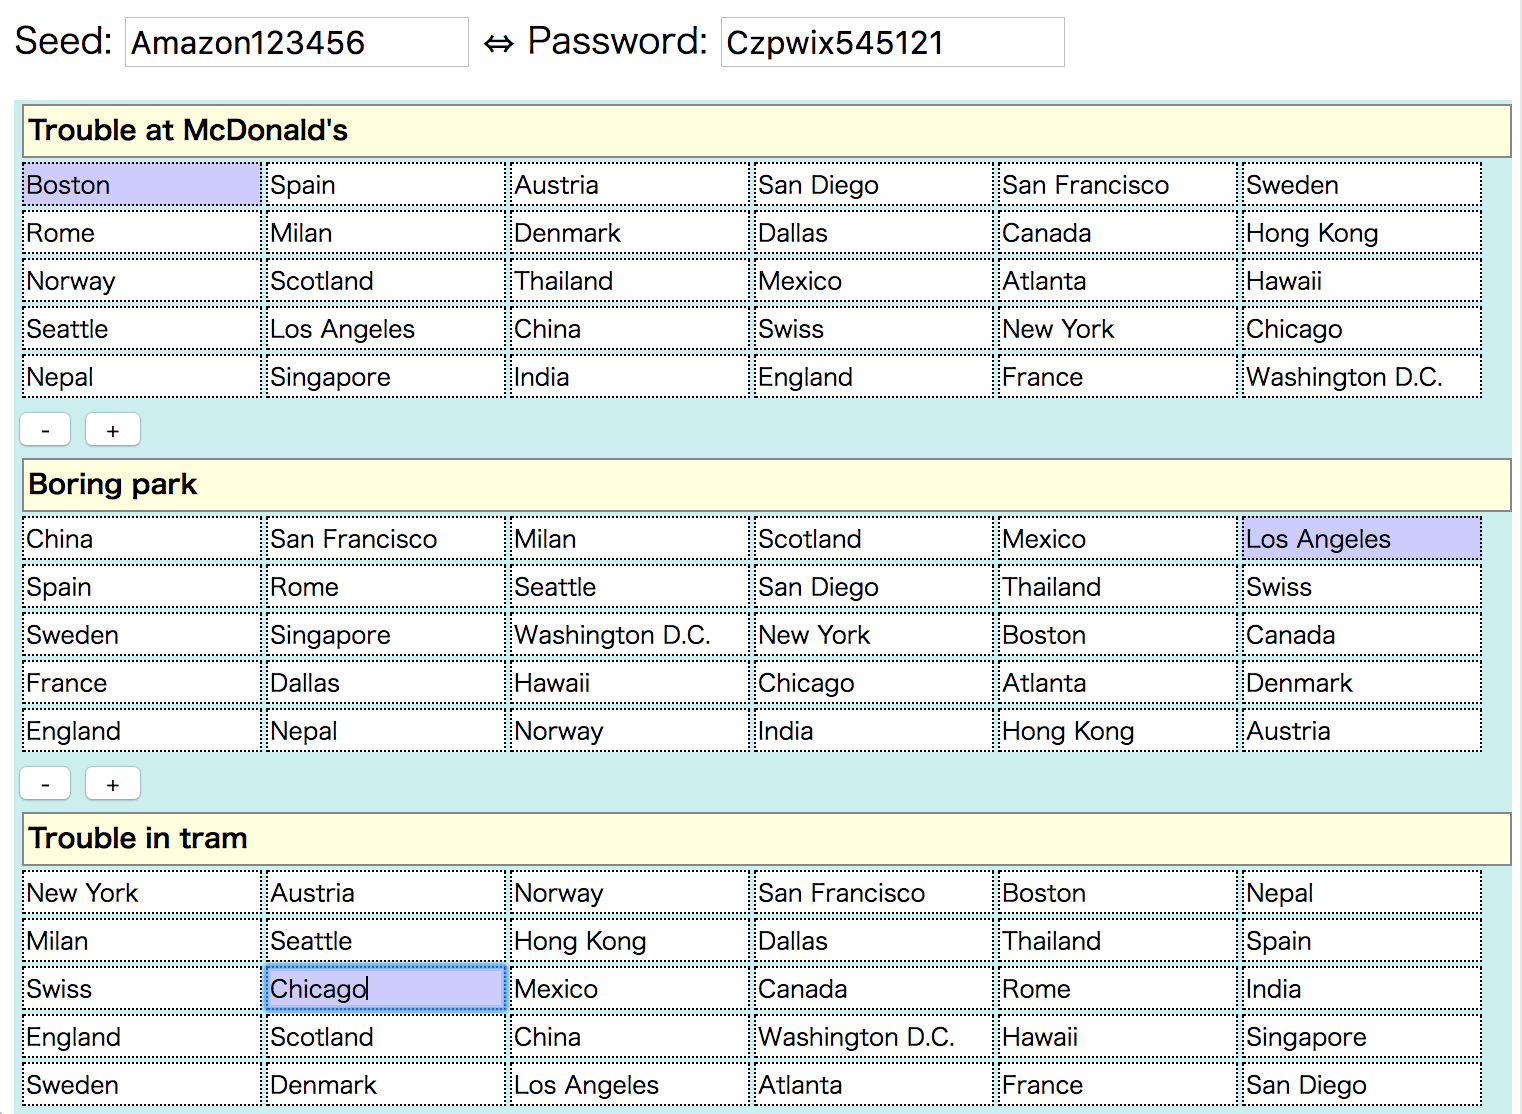
\includegraphics[width=13cm,bb=-250 -100 1272 1014]{figures/EpisoPass0.png}}
  \centerline{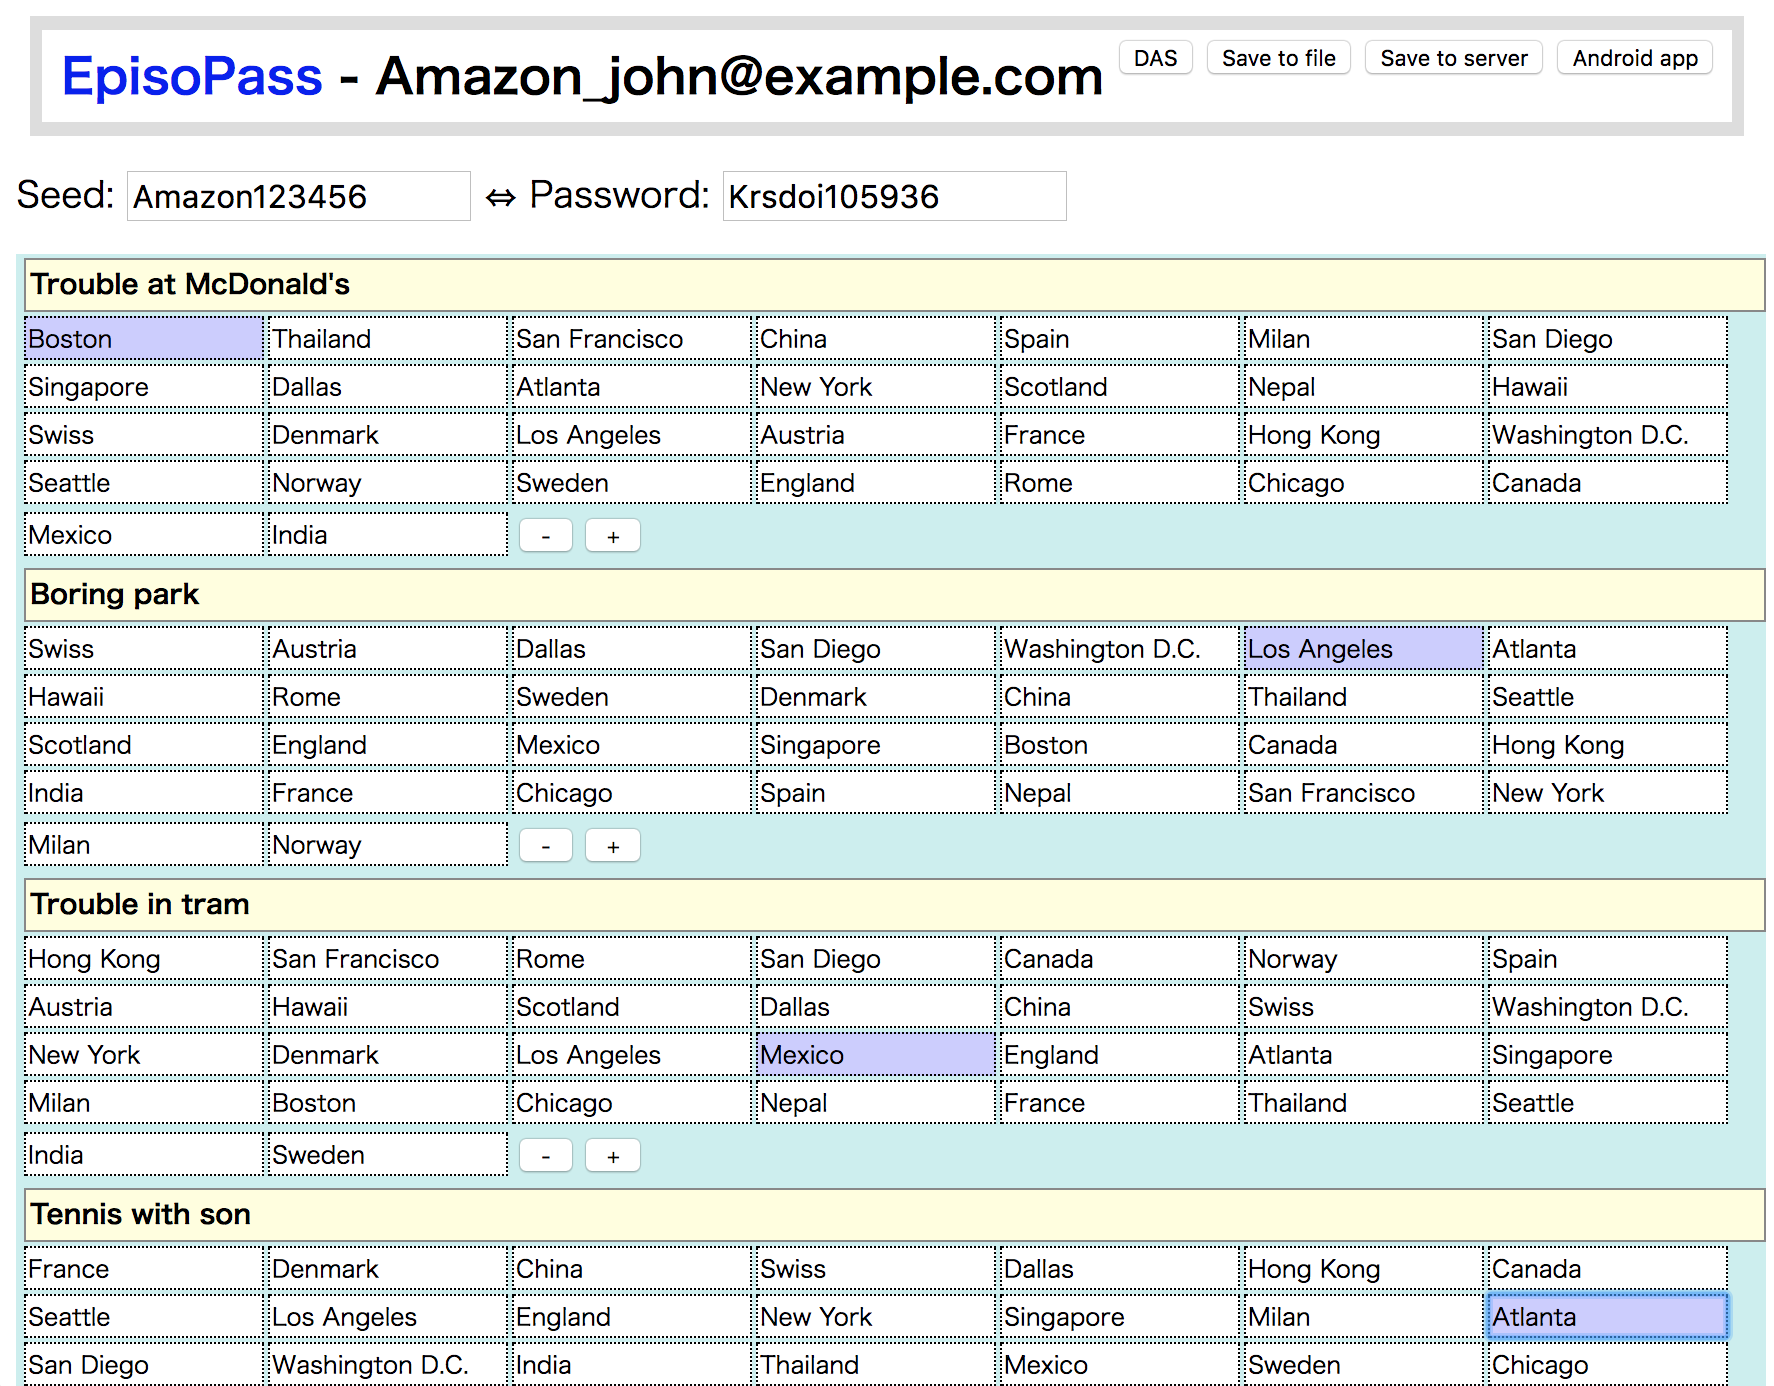
\includegraphics[width=13cm,bb=-250 -100 1524 1286]{figures/EpisoPass1.png}}
  \caption{An EpisoPass page for \textsf{John@example.com}. John can edit questions and answers, enter a seed string,
  and a password is generated based on the selections.}
  \label{EpisoPass}
\end{figure}

Password generation on EpisoPass is performed through the following steps:

\begin{enumerate}
\item A user registers multiple question texts related to their own personal
secret unforgettable episodic memories. For each question they must provide
a single correct answer and multiple additional incorrect answers.

\item The user provides a long ``seed string'' for each service that requires
a password.

\item EpisoPass shows the questions and answers to the user allowing
them to select the correct answer for each question.
Based on the user's selections,
EpisoPass substitutes characters in the seed string and generates a
strong password candidate string.
After selecting all of the correct answers,
the user copies the calculated string
and uses it as the password for the service.
\end{enumerate}

The biggest advantage of using EpisoPass is that
users don't have to remember strong password strings.
%
Users of EpisoPass can save the questions and answers
wherever is convenient. They can
then easily generate passwords by running
EpisoPass and answering the questions.
%
If a question is based on old unforgettable episodic memory,
there is little chance of losing the password for a service
as long as the seed string and questions are available.
%
Answering to many questions takes much longer time than typing a
remembered password, so people may prefer typing password
rather than using EpisoPass if they have to log in to a service frequently.

For the people who don't like to use passwords for authentication,
various types of authentication methods have been proposed.
Especially, visual authentication methods
like graphical passwords \cite{Biddle:2012:GPL:2333112.2333114}\cite{GraphicalPasswords}
and Draw-a-Secret (DAS) \cite{Jermyn:1999:DAG:1251421.1251422} are promising approaches, because
people can remember visual patterns easier than passwords.
%
Visual authentication methods have better characteristics than
password-based authentication, but
they are sometimes fragile to attacks or memorization is difficult.

We propose a new visual password generation system \textit{EpisoDAS}
that posesses the advantages of both EpisoPass and DAS-based methods.

\begin{figure}[t]
  % 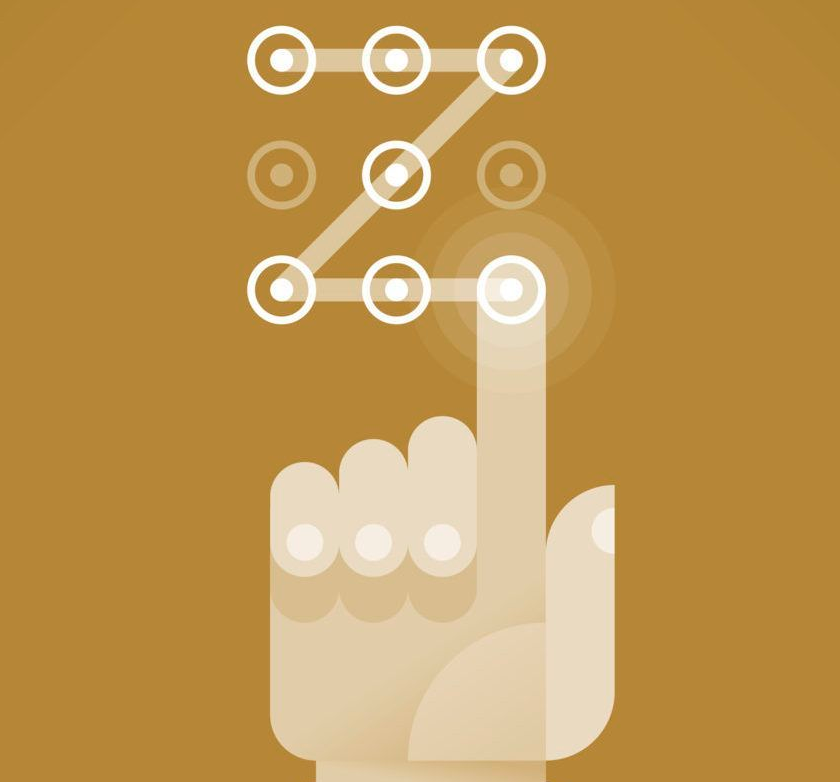
\includegraphics[width=8cm,bb=0 0 840 792]{figures/DAS.png}
  % 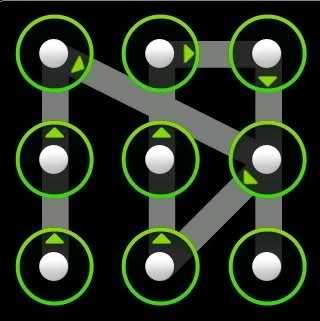
\includegraphics[width=8cm,bb=0 0 320 321]{figures/DASexample.jpg}
  % 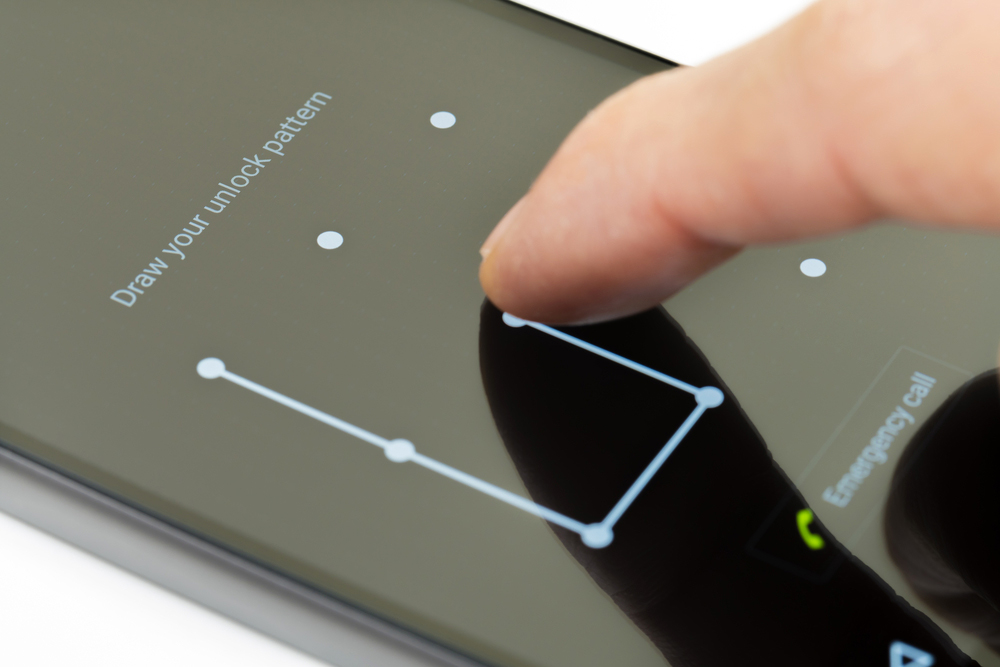
\includegraphics[width=10cm,bb=0 0 1000 667]{figures/AndroidLock.jpg}
  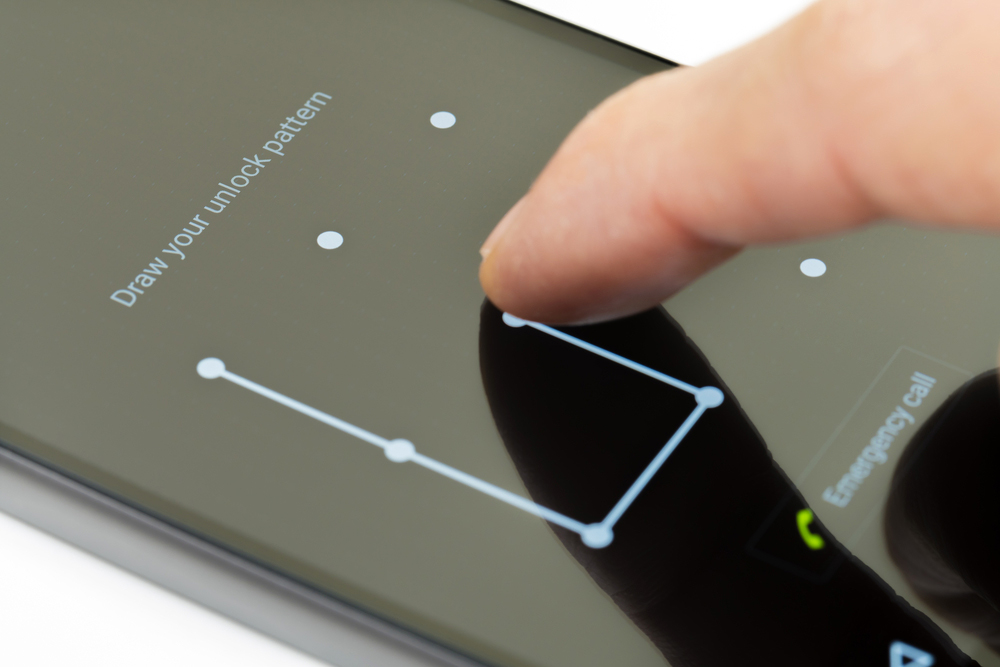
\includegraphics[width=10cm,bb=-60 0 940 667]{figures/AndroidLock.jpg}
  \caption{An example DAS system. (``Pattern lock'' for Android)}
  \label{AndroidLock}
\end{figure}

\section{EpisoDAS}

EpisoDAS is a visual authentication interface
based on the user's episodic memories.
Like EpisoPass,
EpisoDAS displays a list of questions to the user,
asks the user to choose the most appropriate answer from the candidate answers,
and generates a password string based on the user's selections.
%
% with which users can generate strong password based on their
% memory of visual patterns and episodic memories.
% Users can either select answers based on the user's secret episodic memories or
% draw a secret pattern represented by the pattern of selected answers.
% 
% Thus, users can recognize EpisoDas as a DAS system or
% use it as an implementation of EpisoPass.
%
The candidate answers are shown to the user as a grid of buttons,
and the user can select the most appropriate answer to each question
by clicking one of the buttons in the grid.
%
If the location of the series of correct answers form a special
pattern that the user can remember, the user can select
correct answers quickly just like using other DAS systems.

% http://episopass.com/Amazon_john@example.com/Amazon123456
% http://episopass.com/Amazon_john@example.com.html

\begin{figure}[t]
  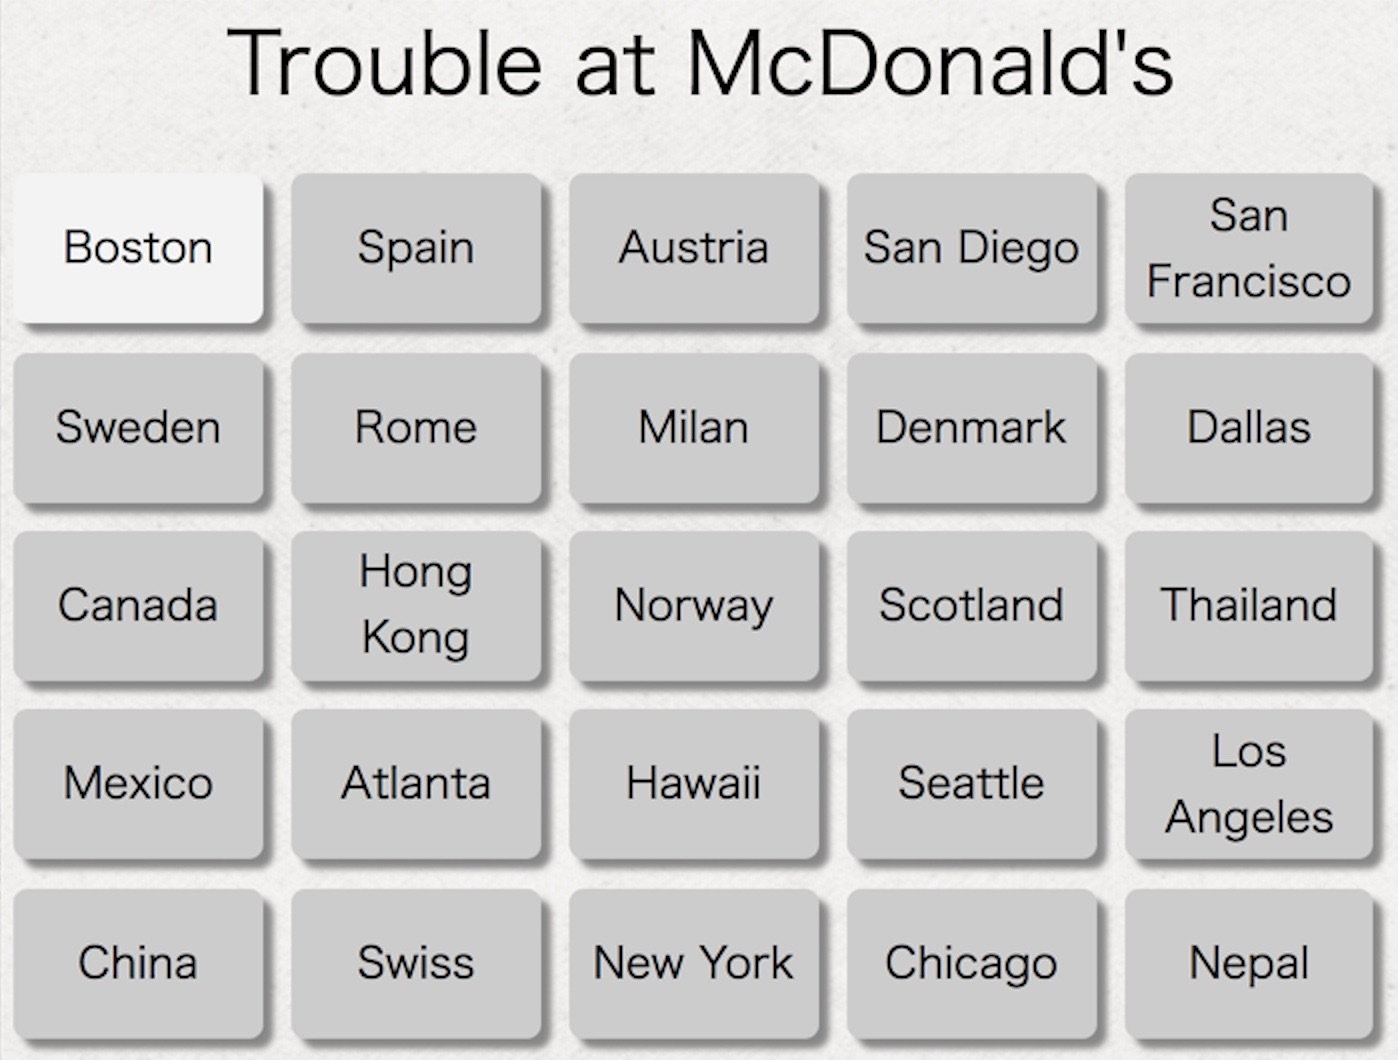
\includegraphics[width=10cm,bb=-60 0 1338 1060]{figures/EpisoDAS1.jpg}
  \caption{First question and candidate answers shown on EpisoDAS.}
  \label{EpisoDAS1}
\end{figure}

Figure \ref{EpisoDAS1} shows
the initial screen of an EpisoDAS session.
% how a user can generate a password from his episodic memories.
%
If the user remembers that he had trouble at a MacDonald's in Boston in the past,
he would click ``Boston'', and the next question (Figure \ref{EpisoDAS2}) is displayed.

\begin{figure}[t]
  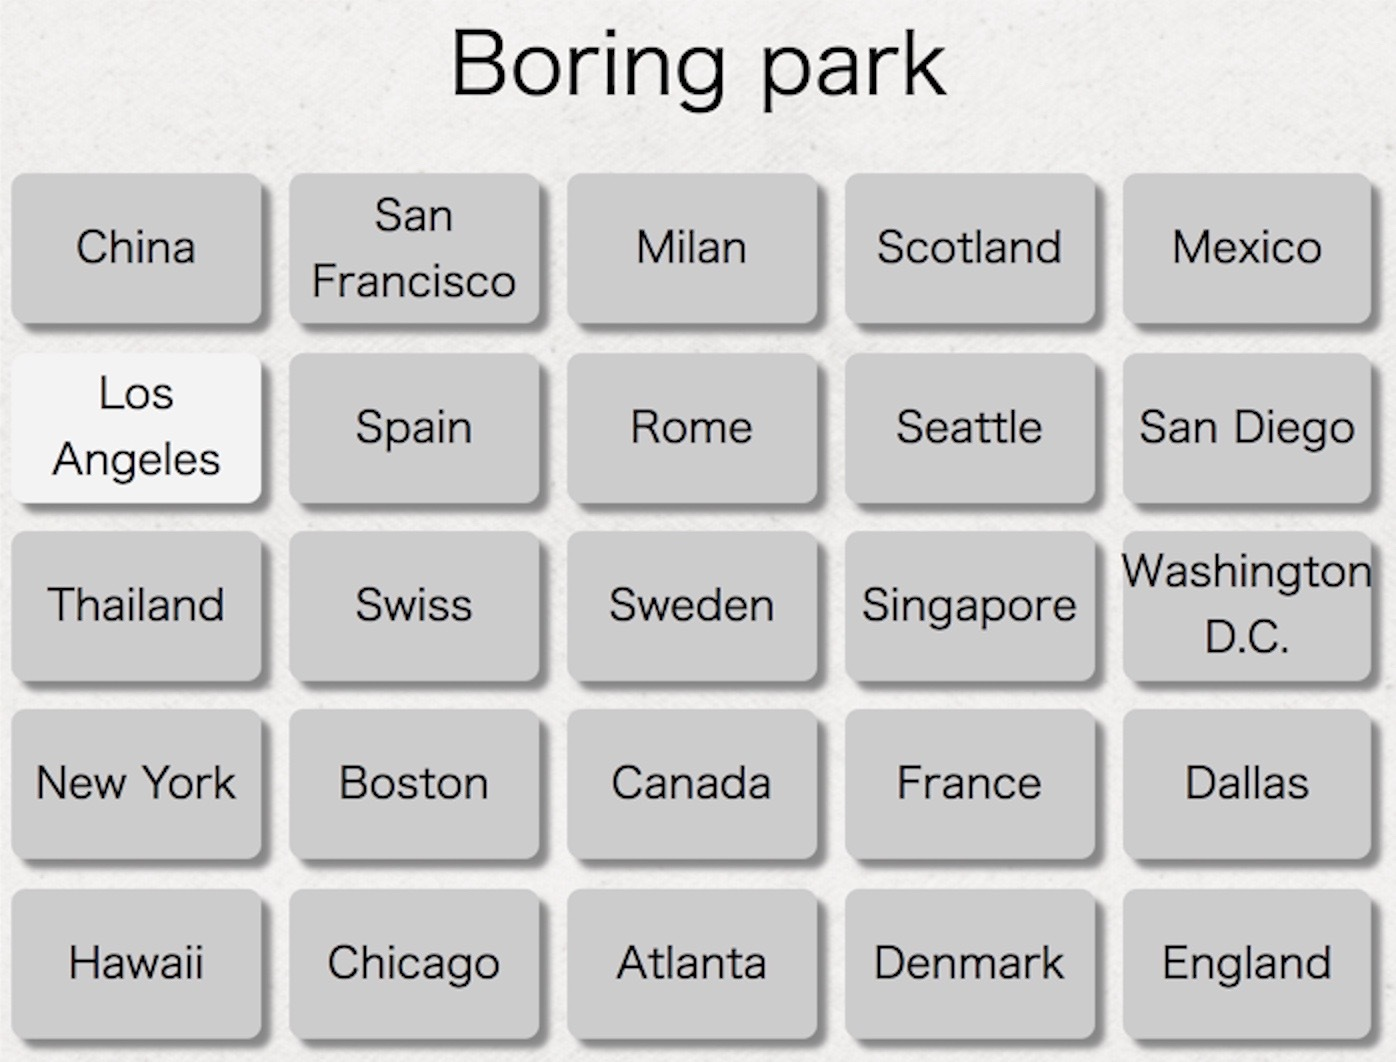
\includegraphics[width=10cm,bb=-60 0 1336 1062]{figures/EpisoDAS2.jpg}
  \caption{Second question and answers.}
  \label{EpisoDAS2}
\end{figure}

If he remembers that he had a bad time at Los Angeles,
% after reading the question in Figure \ref{EpisoDAS2},
he would click ``Los Angeles'' and proceed to the third question.

The contents and the order of the questions
do not depend on the user's actions, and
the user cannot tell whether he has selected a right answer.
%
After repeating the slection process ten times,
the user can get his password
calculated from his selections (Figure \ref{Result}).

\begin{figure}
  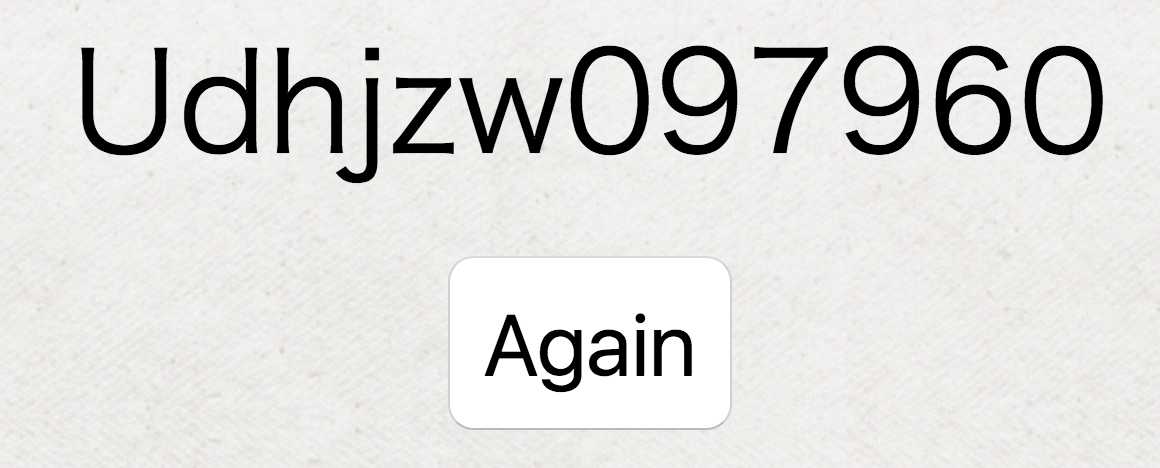
\includegraphics[width=10cm,bb=0 0 1160 468]{figures/result.png}
  \caption{Generated password.}
  \label{Result}
\end{figure}

Users can select correct answers not only by clicking each button,
but by draggin the pointing device on the buttons.
%
If the series of button locations form a special pattern,
% If the series of buttons are aligned next to each others,
the user can drag the pointing device like
Figure \ref{draw} instead of clicking ten buttons,
and quickly generate a password.
%
The order of the list of candidate answers change according to the
drag or click action,
and the user can mix the dragging and clicking actions at any point.
The user can either click ``Boston'' and ``Los Angeles'' one by one or
click on ``Boston'' and drag the pointing device downward to select
``Los Angeles'' without releasing the mouse button or releasing the
pen or finger from the surface of the tablet computer.

\begin{figure}[H]
  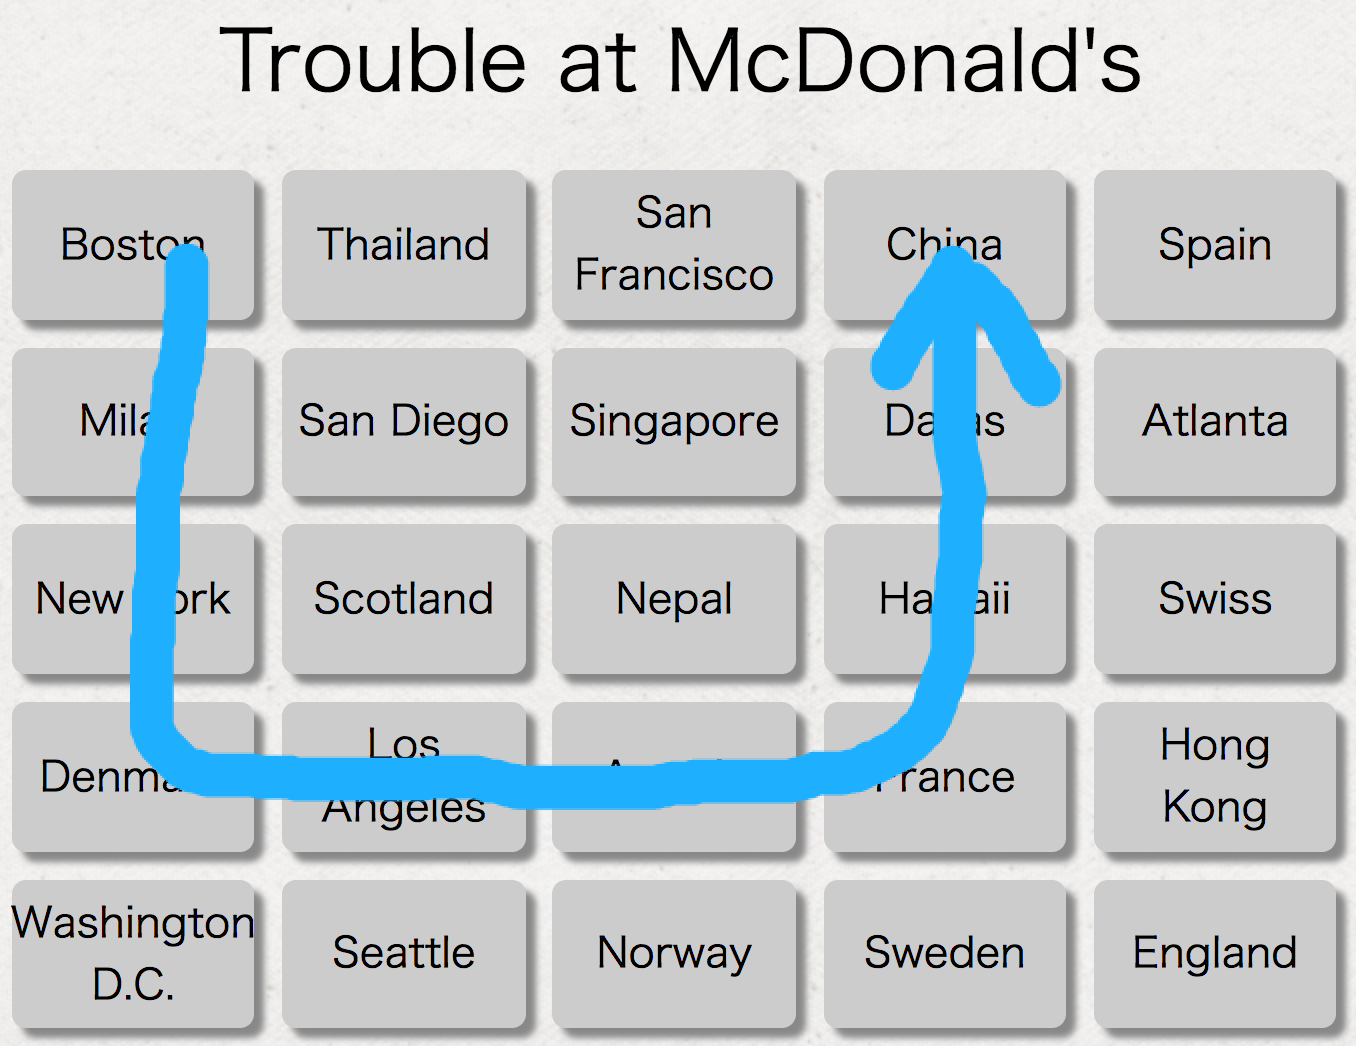
\includegraphics[width=12cm,bb=0 0 1356 1046]{figures/draw.png}
  \caption{Drawing a secret pattern on EpisoDAS.}
  \label{draw}
\end{figure}

The drawing action by the user is close to the actions
used on other DAS systems.
Users can quickly generate his password for authentication
just by drawing a pattern on the EpisoDAS screen.

EpisoDAS can be used for generating passwords for any kind of systems and
services, but it is most useful when it is used to log into a Web service.
Figure \ref{Amazon} shows how a user can use EpisoDAS when
he wants to log in to Amazon.com.
If the EpisoDAS extension is installed on the browser,
an EpisoDAS window appears when a user enters their
email address and clicks the password field.
After selecting answers by drawing a secret pattern on the EpisoDAS area,
a password for Amazon is generated and pasted
into the password field, making the user to log in without typing a password.

% Figure \ref{Amazon} shows how a user can use EpisoDAS on a login page,
% using a browser extension software.
% The extension shows a EpisoDAS window when a user tries to log into
% an Web service, and after the user selects the right answers,
% a password is generated from the input and pasted in to the
% password text box.

\begin{figure}[t]
  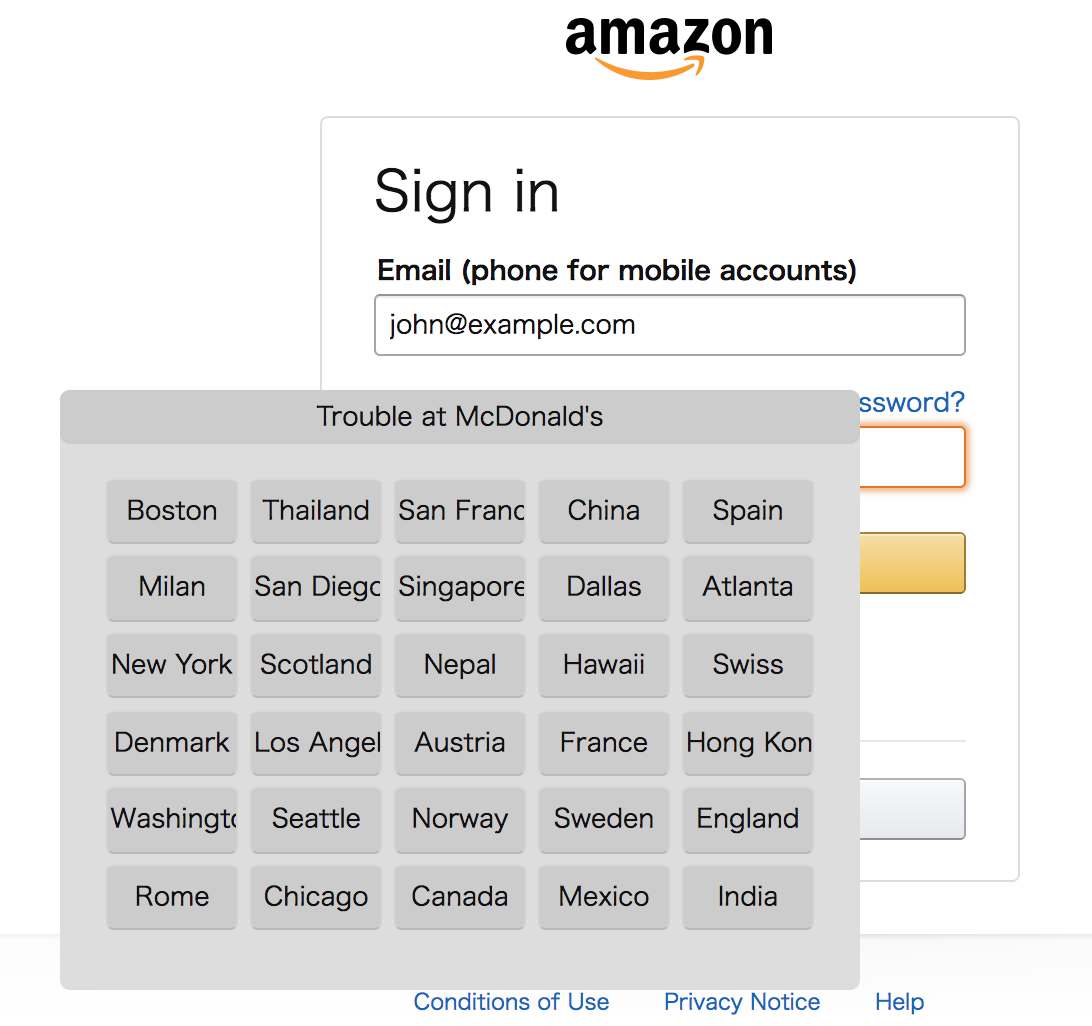
\includegraphics[width=12cm,bb=0 0 1092 1026]{figures/Amazon.png}
  \caption{Using EpisoDAS on Amazon.com login page.
    When the user clicks the password field, EpisoDAS window automatically appears
    and a password is generated and pasted to the field after drawing a
    secret pattern.}
  \label{Amazon}
\end{figure}

The data used in the above example is retrieved from the EpisoDAS database
on the Web, using the name of the service (\texttt{Amazon})
and the user id (\texttt{john@example.com}).

\section{Data Registration}

A user has to register a DAS pattern and
Q-A database before using EpisoDAS.

\subsection{Registering a DAS pattern}

EpisoDAS is based on the EpisoPass system,
and questions and answers should be registered on the EpisoPass database.
After registering questions and answer candidates,
a user can register a DAS pattern so that
answer candidates are easily selected on EpisoDAS.

% \begin{figure}[H]
%   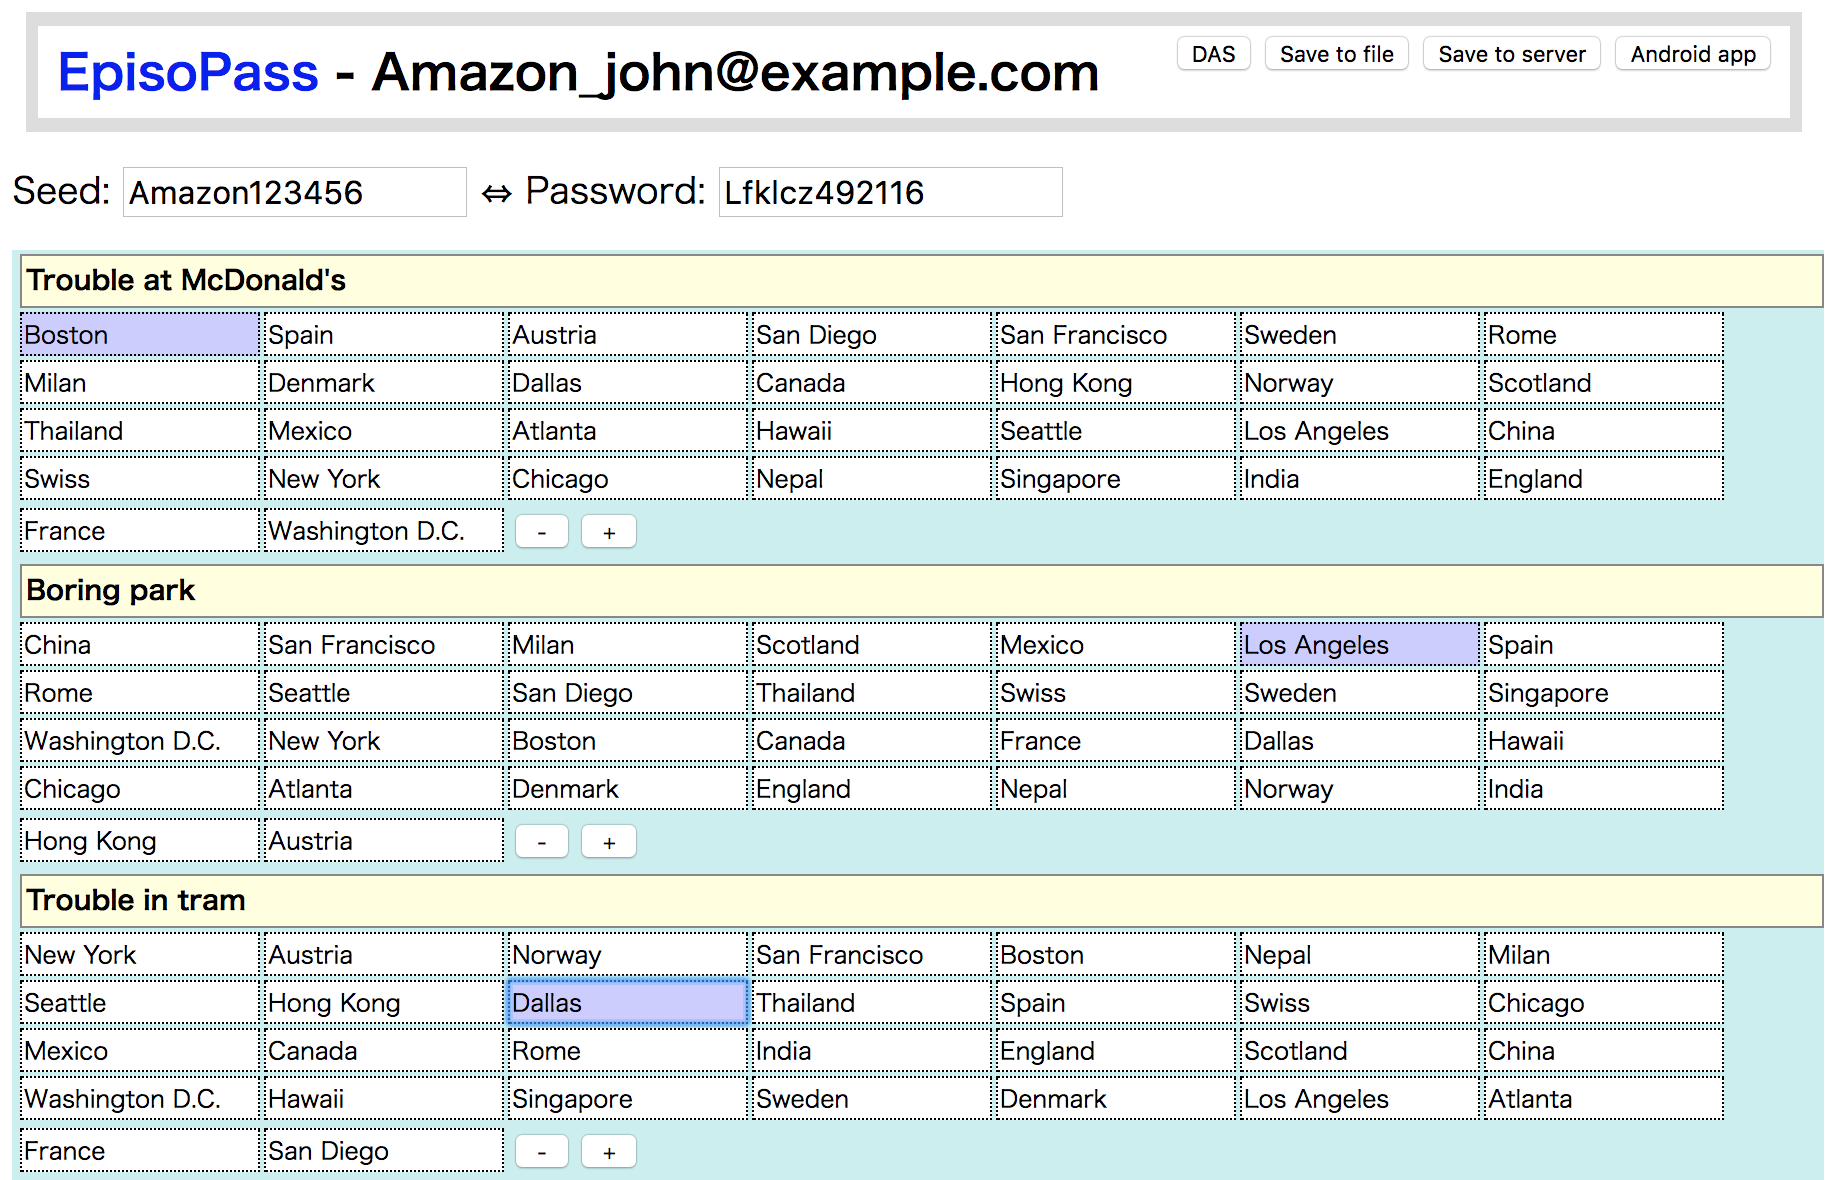
\includegraphics[width=12cm,bb=0 0 1832 1180]{figures/JohnEpisodes.png}
%   \caption{EpisoPass window}
%   \label{JohnEpisodes}
% \end{figure}

After selecting the correct answers
(``Boston'', ``Los Angeles'', etc.) on the EpisoPass editor page (Figure \ref{EpisoPass}),
the user can click the ``DAS'' button on the top-right portion of the
page to proceed to specify their DAS patten.

\begin{figure}[H]
  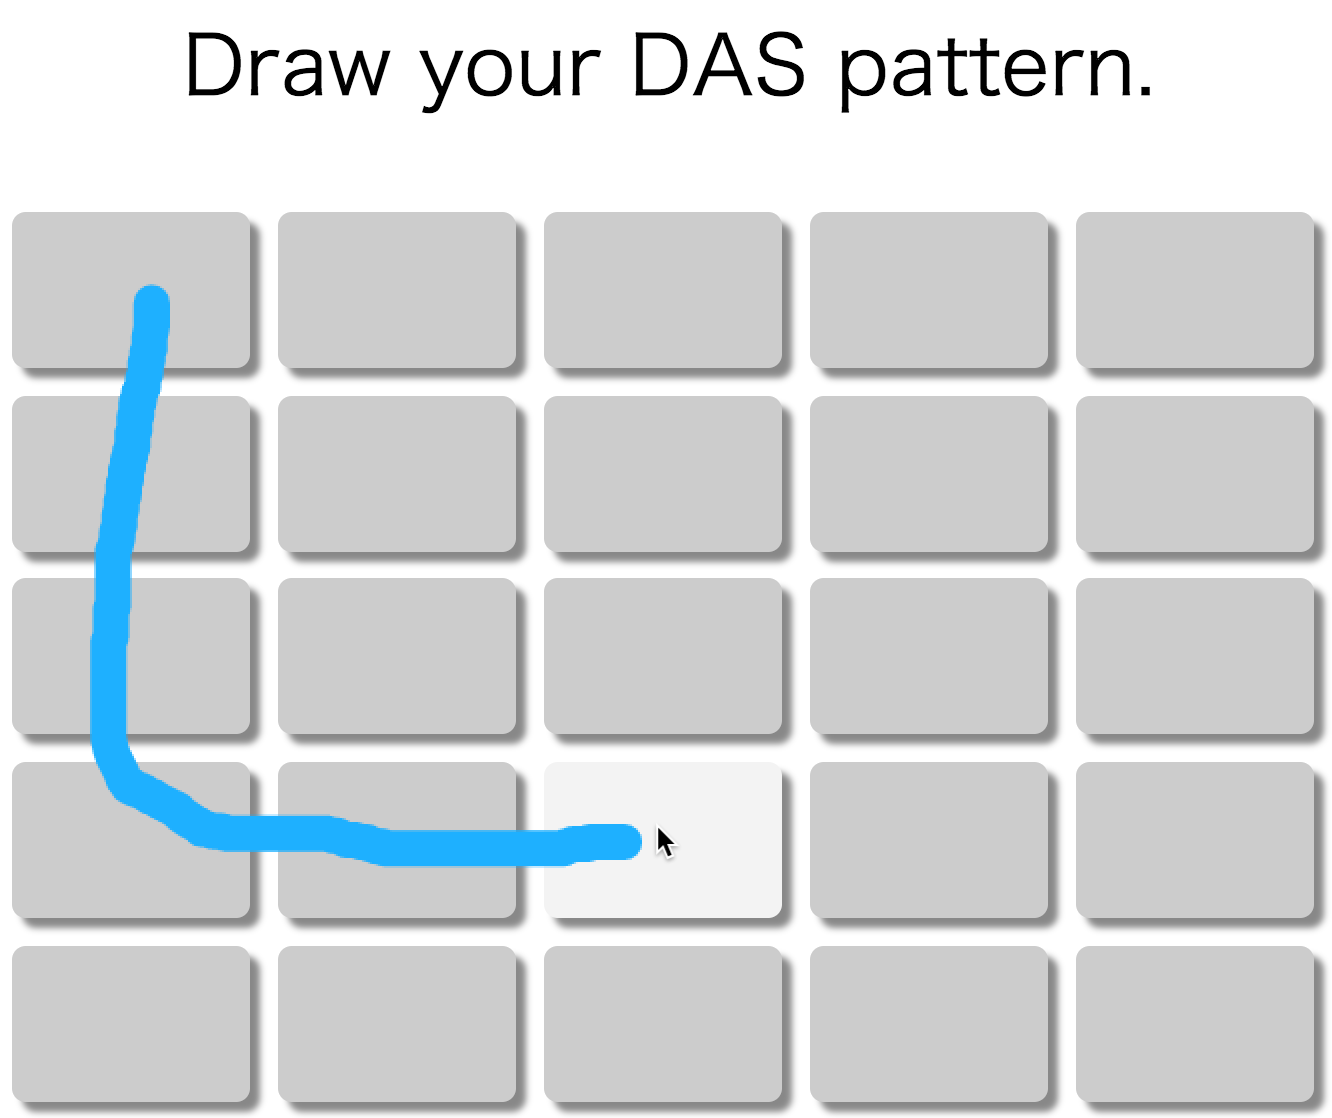
\includegraphics[width=12cm,bb=0 0 1332 1118]{figures/DASRegister.png}
  \caption{Registring the DAS pattern}
  \label{DASRegister}
\end{figure}

If the user wants to use a U-shape as the secret pattern,
he can draw the shape shown in Figure \ref{DASRegister}
on the DAS registration window.
%
After registering the pattern, the candidate answers for the EpisoPass is
shuffled so that the series of correct answers represent the specified pattern.

\subsection{Registering questions and answers}
\label{easyregister}

Questions and answer candidates can be edited interactively on the
EpisoPass editor page (Figure \ref{EpisoPass}) and arbitrary
strings can be specified as questions and answer candidates.
However, creating many questions and answer candidates is
time-consuming and hard task, because
people usually feel it difficult to recall old secret episodes.
%
To help people easily create EpisoPass questions and answers,
a support page can be used for easy problem creation
(Figure \ref{Easy}).

\begin{figure}[H]
  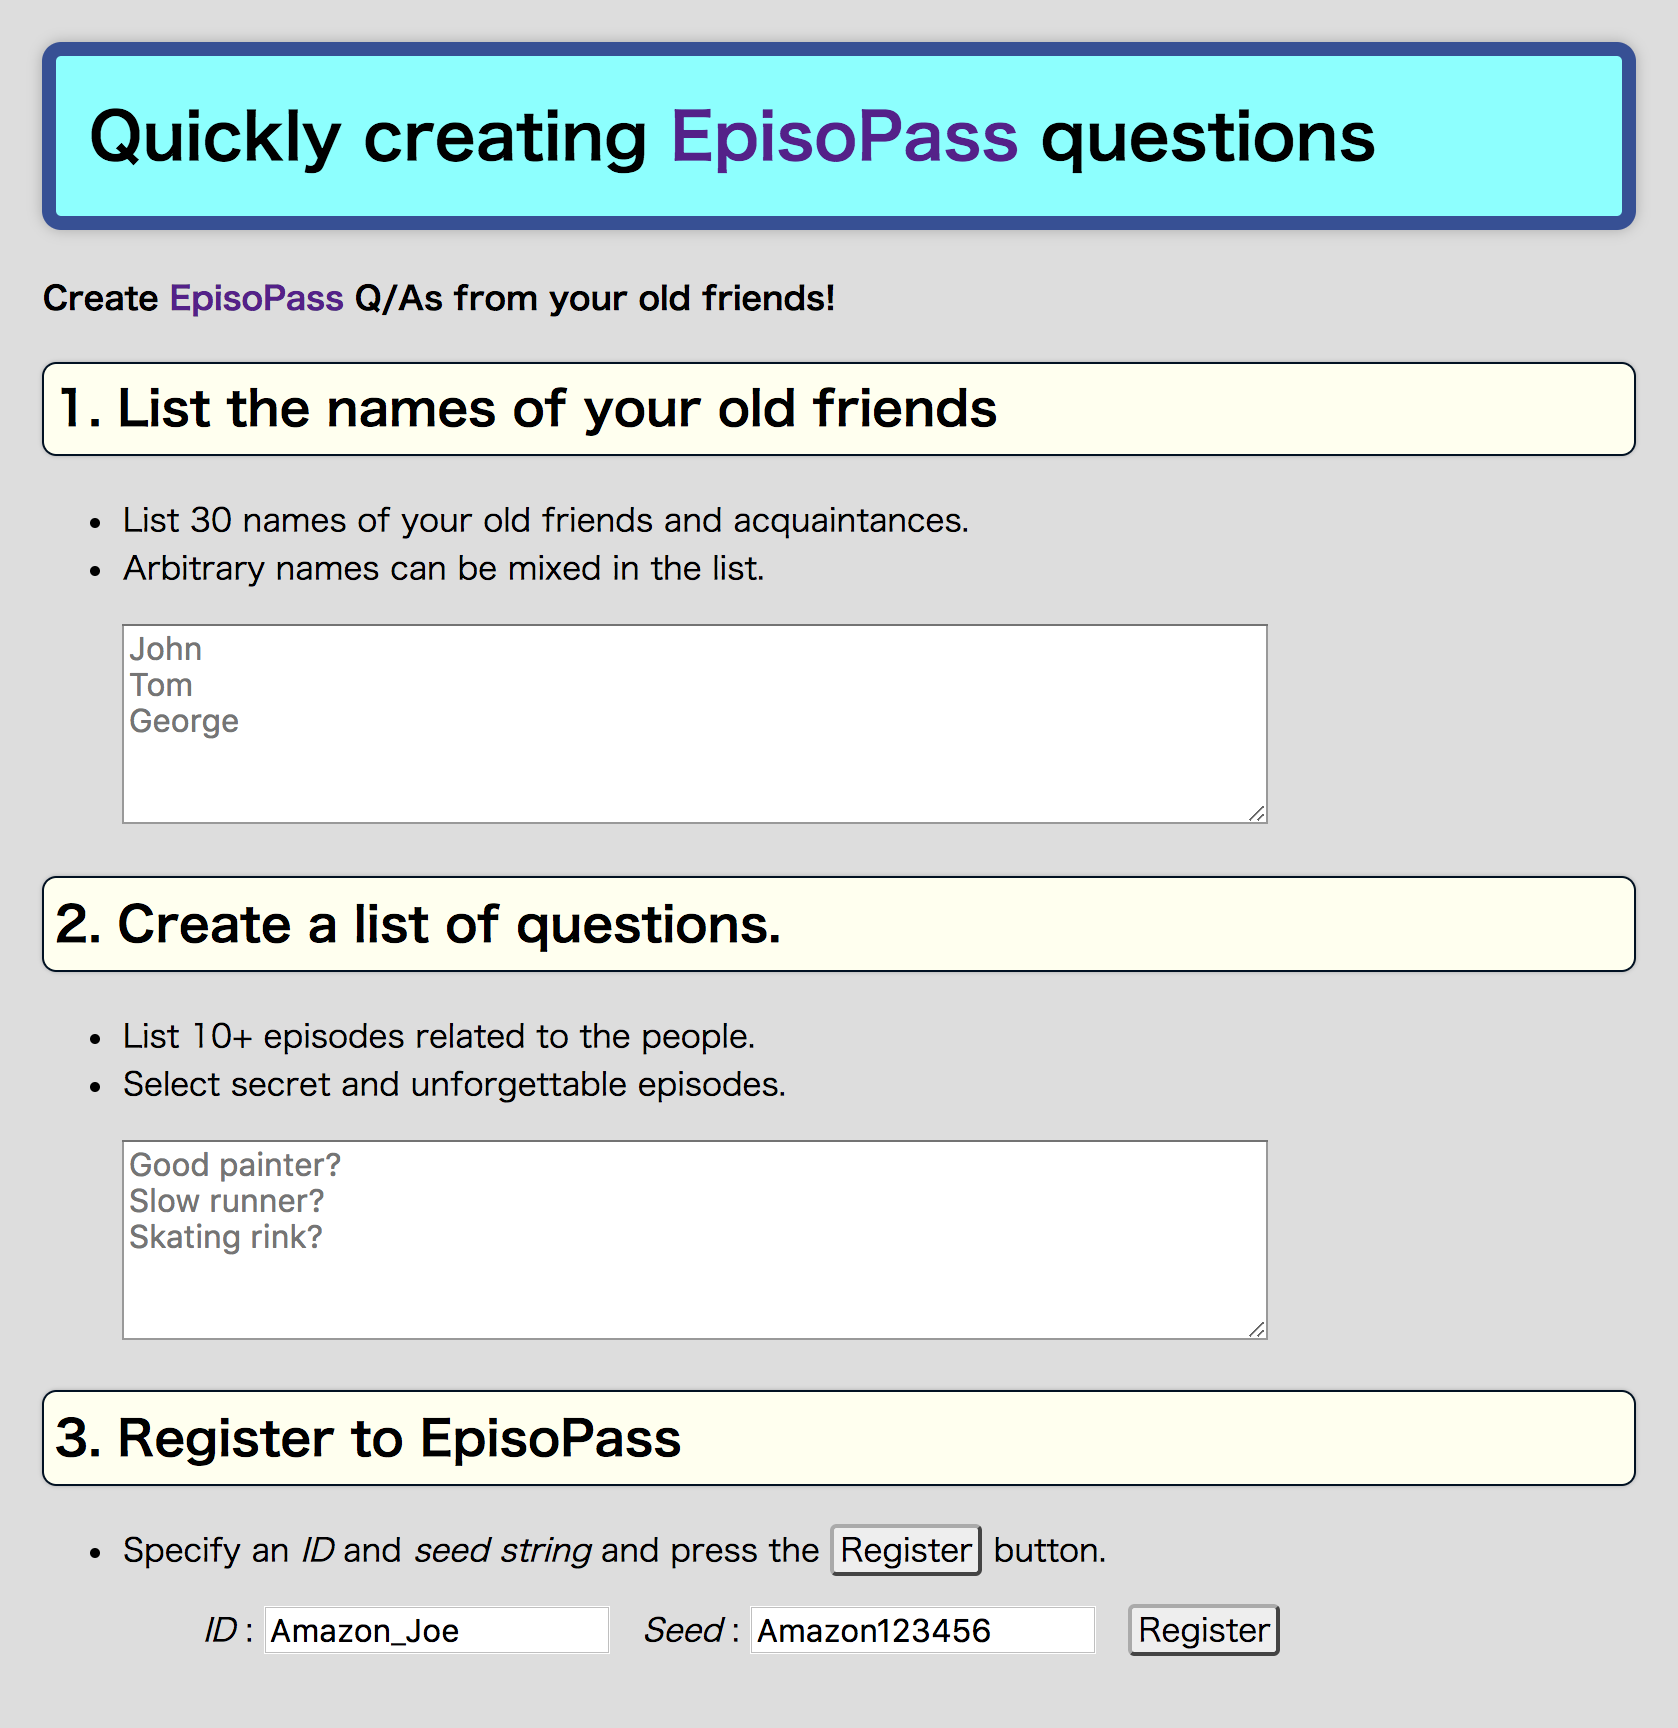
\includegraphics[width=12cm,bb=0 0 1678 1728]{figures/Easy.png}
  \caption{Easily creating questions and answers}
  \label{Easy}
\end{figure}

First, a user provides a list of names of his old friends and acquaintances.
After registering a list of such names,
the user is asked to enter special episodes of the people.
For example, if the user remembers that Tom was
very good at drawing, he can add a question
``Good painter?'' to the list, assuming Tom is the correct answer.

Recalling special old episodes is sounds hard for many people, but
recalling an attribute of an old friends is much easier.
The questions and answers shown in Figure \ref{EpisoPass} was
created by this system,
using place names instead of people's names.

\section{Discussion}

The authors have been using EpisoPass for more than 5 years, and
using EpisoDAS for about an year.
No formal evaluation has been performed so far, but
some people around the authors are enthusiastically using
EpisoDAS for their daily work, and
important impressions have been observed during the period.

\subsection{Authentication time}

Unlike EpisoPass,
very small amount of time is required for
the authentication process on EpisoDAS.
For a skilled computer user,
selecting answers based on the secret might be a little bit slower than
typing a password on a computer with a hardware keyboard, but
authentication with
EpisoDAS is apparently faster on smartphones and tablet computers
than entering passwords on such devices.

\subsection{Forgetting factors}

The biggest advantage of using EpisoPass is that users don't have to
remember long password strings.
%
After the authors began using EpisoPass,
they have been having no problem forgetting passwords of any kind.
%
As long as a user have the seed string and question-answer data,
he can easily generate passwords by running
EpisoPass and answering the questions.
%
If the questions are based on old unforgettable episodic memory,
there is little chance of losing the password for a service
as long as the seed string and questions are available.
%
If the user's memory is related to an episode that took place 20 years
ago, say, and the user clearly still remembers the episode now, it is
unlikely the episode will be forgotten in the future.

% The seed string and question-answer data can be put on a public place
% if they include enough amount of secret information.

\subsection{Running environment}

EpisoDAS is implemented as a single HTML file that includes a JavaScript
script for password calculation.
The HTML file can be put on the Web or saved in a handy USB memory device
so that it can be accessed from a Web browser.
%
If the questions are based on the user's secret memories and
a sufficient number of questions and fake answers are provided,
the data can be put on a public Web page or saved in a secure
repository like GitHub.
%
The data set of the authors are put on the Web, and it can be easily
found using Web search engines\footnote{
  The EpisoDAS data of the authors can be found on major Web
  search enginges using the name of the author and ``password''.
}.
It means that the passwords used by the authors can be retrieved
even when the data is not available locally.

\subsection{Universality}

Using EpisoDAS, people can use password-based systems
only by selecting answers based on their episodic memories,
without remembering passwords or using password management systems.
Using a browser extension,
people can use services without noticing that passwords are
required for the service.

Creating a Q-A database is a one-time process,
after which the system becomes straightforward to use.
%
With a proper help, creating a database is not difficult even for
people who are not good at using computers.
A helper can ask the client questions like
``Do you remember an interesting friend in your childfood?''
to get the list of old friends, and then ask questions like
``What kind of child was he?'', ``Do you remember his house?''
to create a question for locating him.
With such information, the helper can use the technique shwon
in Section \ref{easyregister} to create the EpisoDAS database
for the client.

\subsection{Security strength}

The strength of the generated passwords depends on the number and 
level of secrecy of the questions.
%
There have been many studies on the strength of passwords
\cite{Hayashi:2011:DSP:1978942.1979326,Komanduri:2011:PPM:1978942.1979321}, % What password is strong
but measuring the strength of secret questions is an area where more study is needed.
% \marginnote{I calculate $20^{10} = 10,240,000,000,000$. This is
% considerably more than a billion (closer to 10 thousand billion,
% (US) or 10 million million (UK).}
Using ten secret questions each with twenty answers, where each answer is considered equally likely,
an attacker would need to cover a search space of over ten trillion ($20^{10}$) values to check
every potential combination of answers,
and the entropy of the system is 43.2 ($10 \times \log_2 20$) bits.  % 10.0 * (Math.log(20.0)/Math.log(2.0))
%
This represents roughly the same entropy as using a random 8-character Latin-alphabet
password, for which the entropy is 45.6 bits.
This level is considered to be strong enough for Web services,
where it's not possible to perform online brute-force attacks \cite{Florencio:2007:SWP:1361419.1361429}.
  
\subsection{Choosing questions}

The quality of the questions is key to using EpisoDAS effectively.  If
the episode is shared by someone else, this other person might easily
be able to answer the question and generate the user's password.
%
The episode related to each question should therefore not be known to any other person,
and the episode should be unforgettable.
%
Finding such episodes seems difficult at first,
but using the method shown in the last section,
it is not extremely difficult to recall
many trivial episodes which are unforgettable but
nonetheless not important to other people.

Questions such as ``Who did you like best?'' should be avoided,
since friends or family might know the user's tastes, thereby allowing 
others to select the correct answer.
Also, memories related to taste is more fragile than fact-based memories like
``Where did you find a crystal?''.

% \subsection{Question reuse}
% 
% 使い回しが駄目
% どこかのサイトのパスワードが流出し、
% そのEpisoPassデータが公開されていたら
% ブルートフォースで答がわかってしまうから
% 問題を使い回すことは好ましくない

\subsection{Developmenet of browser extensions}

EpisoDAS browser extension is very useful, but creating the extension
is cumbersome because there is no standard login form for
Web services.
%
The browser extension should first detect that the Web page is a login page
of a Web service (e.g. Amazon),
and then it should be able to get the ID of the user
and know where the result of EpisoDAS calculation should be pasted.
%
Commercial password managers\cite{OnePassword,Dashlane,LastPass,KeyPass,NortonIDSafe,IDManager}
are usually well integrated with Web browsers,
and EpisoDAS should also be evolved so that
the browser extension works on many Web services.

\subsection{Battles against sholder surfing}

Simple DAS authentication is known to be vulnerable to ``shoulder surfing''
attacks\cite{Aviv:2017:TBS:3134600.3134609}.
If the secret pattern is simple and
the pattern can be easily observed over the user's shoulder,
attackers can easily reproduce the login pattern.

This problem is common to all the DAS-based authentication systems,
and great care should be taken when drawing a secret in the public.
EpisoDAS users can use more complex DAS patterns than
conventional DAS systems,
because there is no risk of forgetting the pattern,
since the user can read the question at any time and
remember the secret pattern which corresponds to the
answers to the questions.

\subsection{Risks of Forgetting DAS pattern}

Using a conventional DAS system, users should be carefull about
remembering the DAS pattern.
DAS patterns may be more easily remembered than password texts,
but there is always some risks about forgetting them.
Using EpisoDAS, users can easily remember the DAS pattern
just by reading the questions and answers.
Users can be very sure that they will never forget the pattern,
because the pattern can be retrieved by answering the questions.

EpisoDAS is the combination of EpisoPass and DAS-based authentication methods.
A user can generate a password using his episodic memories, or
he can generate a password using the DAS pattern he remembers.

\section{Conclusions}

We introduced a password management system \textit{EpisoDAS}
that generates a password from a seed string by
quicly drawingn a secret pattern backed by the user's episodic memories.
These memories are represented as a set of questions and answers
which can be solved only by the user in order to generate a site-specific password.
%
Using EpisoDAS, a user can log into Web services quickly without
worrying about
having to remember any secret information, other than the episodic memories
that have been chosen specifically to be easy to recall.
%
We are hoping to make EpisoDAS available on all the environments
where strong passwords are required, and
relieve everyone's pain of password handling.

\large
\bibliographystyle{ACM-Reference-Format}
\bibliography{paper}

\end{document}
